\paragraph{Linear mechanisms}
One research group explores the repelling two magnets and a latch to keep the braille character in place \cite{kim_braille_2020} with reasonable results.
It is also possible to use attractive forces to depress the braille character \cite{bettelani_design_2020}.
The mechanism relies on using a solenoid to generate a magnetic field that moves downwards a ferromagnetic element that is surrounded by a spring.
When current stops being applied, the spring extends and pushes the braille pin up.
This setup is shown in figure \ref{fig:magnetic-spring.png}.
This model is safe, simple to replicate and the cheapest solution with an estimated cost of USD 40 per cell \cite{bettelani_design_2020}.
Besides, it also has the potential to be converted into large area dense array display, which satisfies our goal. 

\begin{figure}[h] \centering
    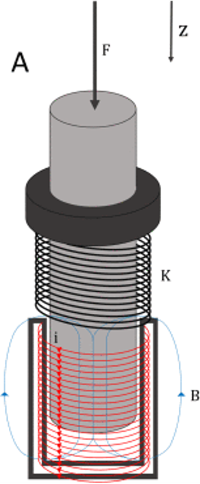
\includegraphics[height=5cm]{figures/magnetic-spring.png}
\caption[Linear magnetic actuation mechanism]{A solenoid with the ferromagnetic element and the linear spring (elastic constant $k$). A current $i$ flows in the red solenoid and generates a magnetic field $B$. In turn, the force $F$ acts downwards, displacing the bar a distance $z$ \cite{bettelani_design_2020}.}
\label{fig:magnetic-spring.png}
\end{figure}

Generally the technologies used for actuation actively displace the pin out of a socket.
Loconsole et al. \cite{loconsole_braillecursor_2019} explore the use of passive pins and a magnetic rail that pulls each pin, then drops them in a given position that results in up or down. Figure \ref{fig:magnetic-rail} shows this scheme.
While the reduced energy consumption due to passive components is appealing, this solution has a very high error rate of at least 5\%, and each row of cells necessitates a large motor that inhibits the density required by our device.
\begin{figure}[h]
\centering
    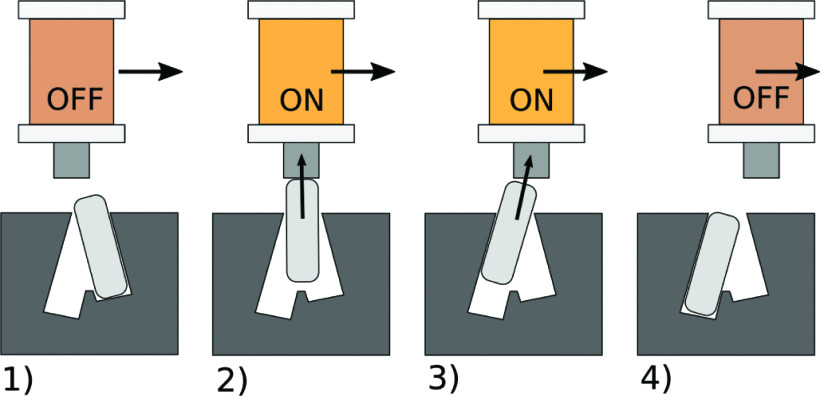
\includegraphics[width=0.6\textwidth]{figures/magnetic-rail.jpg}
\caption[Magnetic rail actuation mechanism]{Magnetic rail actuation mechanism. Pins are magnetically pulled from the socket and deposited in either position, having them be on or off (or up and down)}
\label{fig:magnetic-rail}
\end{figure}  

\paragraph{Ferromagnetic fluids}
Despite its early developmental stage, the use of ferromagnetic fluids is promising \cite{fletcher_magnetic_2021}.
Character in a cell are individually created by their correspondent electromagnet, and can reasonably meet the UK Association for Accessible Formats (UKAAF) standards.
Given it is at a proof-of-concept stage, producing it for this study is unreasonable.